\documentclass[12pt, a4paper]{article}

\usepackage[english]{babel}
\usepackage[utf8]{inputenc}
\usepackage{hyperref, bookmark}
\usepackage{graphicx}
\usepackage{fancyhdr}
\usepackage{mathtools}

% set images
\usepackage{float}

% pseudocode
\usepackage{algorithm}
\usepackage{algpseudocode}

% graphs
\usepackage {tikz}
\usetikzlibrary{positioning}

\usepackage[left=2cm,right=2cm,top=2cm,bottom=2cm]{geometry}

% Images next to each other
\usepackage{subfig}

% citing
\usepackage[square,numbers]{natbib}
\bibliographystyle{dinat}

% general page design
\pagestyle{fancy}
\fancyhf{}
\lhead{Bachelorthesis}
\rhead{University of Hildesheim}
\rfoot{\thepage}

% front page
\title{\LARGE Bachelorthesis\\\large Comparing different state-of-the-art solutions for image prediction using time-series analysis}
\author{ Sören Dittrich\\
	\texttt{\href{mailto:soeren.dittrich@uni-hildesheim.de}{soeren.dittrich@uni-hildesheim.de}}
}
\date{September 2020}

% start of document
\begin{document}
 \bibliographystyle{alphadin}
 
 % Abstract
 \begin{titlepage}
  \maketitle
  \thispagestyle{empty}
  \begin{abstract}\noindent 
   % Abstract
The thesis will compare different state-of-the-art solutions for image-/video-prediction \ref{subsection::imageprediction}.
The main module of the solutions, which is the core aspect of this work, is the LSTM (Long short-term memory) \ref{subsection::lstm}.
This module was invented by Hochreiter and Schmidhuber  \cite{Hochreiter1997} in 1997 and is used heavily in the field of image-\& video-prediction since then, e.g. in Srivastava et. al. 
\cite{Srivastava2015}.
During the time the module got many different add-ons and changes, which are described in different papers (\cite{Patraucean2015}, \cite{Lotter2016}, \cite{Wang2017}, \cite{Wang2018} and many 
more.). To have a valid comparison, I implement three different state-of-the-art solutions for image-/video-prediction (\cite{Shi2015}, \cite{Patraucean2015} and \cite{Lotter2016}).
All of them use the Shi et. al. ConvLSTM \cite{Shi2015} (Or a slightly different version) as recurrent sub-module, which is changed during the experiments
with another, more advanced solution named PredRNN \cite{Wang2017}. The algorithms are re-implemented in PyTorch \cite{Paszke2019}, as well as the \glqq standard\grqq ConvLSTM and PredRNN.
  \end{abstract}
 \end{titlepage}
 
 % Table of contents
 \pagenumbering{Roman}
 \tableofcontents
 \newpage
 \pagenumbering{arabic}
 \setcounter{page}{1}
 
 % question
 % section
\section{Scientific questions}
 \begin{enumerate}
  \item What different types of image prediction architectures exist?
  \item What different types of recurrent modules exist?
  \item How important is the choice of the recurrent module for the runtime and performance of the algorithm?
 \end{enumerate}
 \newpage
 
 % introduction
 % section
\section{Introduction} \label{section::introduction}
 The task of this chapter is to give the reader the basic knowledge, which is necessary to follow the rest of the thesis. In general, the reader should have basic knowledge about machine learning
 and neural networks.
 As this thesis is in the field of machine learning, more explicit neural networks and image-/video-prediction, this chapter will start giving basic knowledge about image-/video-prediction
 and specific neural network architectures, which are used in the thesis.\\\\
 The necessary neural network architectures are Autoencoder~\ref{subsection::autoencoder}, RNN~\ref{subsection::rnn}, LSTM~\ref{subsection::lstm}
 and ConvLSTM~\ref{subsection::convlstm}, they are described briefly for the reader.
 Afterwards I describe the backpropagation algorithm~\ref{subsection::backpropagation} and BPTT~\ref{subsection::bptt} at a very basic level.
 Those two algorithms are the most used algorithms in training neural networks and are used in this thesis. Lastly I describe PyTorch~\ref{subsection::pytorch}, in which I re-implemented the baselines
 for this thesis.

 % subsection
 \subsection{Image Prediction / Video Prediction} \label{subsection::imageprediction}
  Image-/Video-prediction is a field inside machine learning, where the key is to predict future images, given a sequence of images. The image sequence $X$ is of length $n$, ($x_0, \ldots, x_{n-1}$).
  \\\\
  One possible use-case is the \textbf{one-frame prediction}, where one predicts $x_n$, given the the sequence $X$. Another common use-case is \textbf{multi-frame prediction}, where the key is to 
  predict $t > 1$ many frames into the future ($x_n, \ldots, x_{n+t-1}$).
  This is often performed using sequence-to-sequence learning \cite{Sutskever2014}. The first frames will look much better then the last frames, as 
  ground-truth is missing, The predicted frames are only approximated, which means they contain a certain level of error, so using them as input to perform \textbf{multi-frame prediction} will
  increase the level of error for the following frames.

 % subsection
 \subsection{Autoencoder} \label{subsection::autoencoder}
  The autoencoder is a network architecture, which consists of two neural networks chained together. The first network is called Encoder. This Encoder gets the input $x$ and outputs
  the code h. Often the output layer of the Encoder is named bottleneck-layer. The second network is called Decoder. It gets the code $h$ as input
  and outputs $x \prime$. This architecture is used for reconstruction, where $x \approx x \prime$. To prevent the architecture to simply copy the input directly to the output (which would be an
  interpolation and not the goal of any machine learning algorithm.), there are different techniques to have the autoencoder to instead approximate the output.\\\\
  \begin{equation}
   E(x) = h
  \end{equation}
  \begin{equation}
   D(h) = x \prime
  \end{equation}
  \begin{equation}
   D(E(x)) = x \prime
  \end{equation}
  The simplest autoencoder architecture is the so named undercomplete autoencoder \cite{Goodfellow2016}, in which the output of the bottleneck-layer $h$ is smaller then the input $x$.
  Therefore the architecture needs to learn how to extract useful features from the input $x$, because it is not able to simply copy the input $x$ to the output $x \prime$, because $h$ is a reduced
  representation of $x$. There are many different ideas of using the autoencoder architecture, which are described more in-depth in e.g. Goodfellow et. al. \cite{Goodfellow2016}.
  \begin{figure}[H]
   \includegraphics[width=0.35\textwidth]{../Images/autoencoder_schema.png}
   \centering
   \caption{Autoencoder schema \cite{wiki2019}}
   \label{fig:lstm_architecture}
  \end{figure}

 % subsection
 \subsection{RNN} \label{subsection::rnn}
  RNN (Recurrent neural network) is a network type, which is able to handle sequential data $X = (x_0, \ldots, x_{t-1})$, $|X| = t$. Therefore this type of network is used for e.g. time-series 
  analysis and image-/video-prediction~\ref{subsection::imageprediction}.\\\\
  Despite a standard feed-forward neural network, a RNN will not only get a new input at a time-step, but also the output
  of the RNN of the last time-step. This requires a RNN to be initialized at start, because there is no output of the last time-step available. This last time-step input is often initialized as $0$.
  A standard feed-forward neural network looks like:
  \begin{equation}
   \hat{y} = f_{\theta}(x)
  \end{equation}
  Every approximated output $\hat{y}$ is only dependent of the input $x$ and the computation inside the network.
  The RNN looks like:
  \begin{equation}
   \hat{y^t} = f_{\theta}(\hat{y^{t-1}};x^t) = f_{\theta}(f_{\theta}(\hat{y^{t-2}};x^{t-1});x^t) = \ldots
  \end{equation}
  The approximated output $\hat{y^t}$ depends on the input $x^t$, but also on all previous outputs.
  In the literature the RNN is often schemed using a folded and an unfolded graph, to illustrate how the network architecture works.
  \begin{figure}[H]
   \includegraphics[width=0.8\textwidth]{../Images/rnn.png}
   \centering
   \caption{RNN schema \cite{Olah2015}}
   \label{fig:lstm_architecture}
  \end{figure}\noindent
  The output of a RNN is often denoted as $h$ for hidden-unit, because it is not only the output of the time-step, but also the input for the next time-step. \label{sentence::hidden}\\
  This networks are not learned with simple backpropagation~\ref{subsection::backpropagation}, but often with BPTT (Backpropagation through time)~\ref{subsection::bptt}.
 
 % subsection
 \subsection{LSTM} \label{subsection::lstm}
  LSTM (Long Short-term Memory), invented by Hochreiter and Schmidhuber \cite{Hochreiter1997} is a form of RNN, which avoids a critical problem of standard RNN: Saving 
  \textbf{Long-term dependencies} 
  \cite{Goodfellow2016}.
  The architecture consists of different submodules: An inpute-gate, forget-gate, cell-state and output-gate.
  \begin{equation}
   i_t = \sigma(w_{x_i}x_t + w_{h_i}h_{t-1} + b_i)
  \end{equation}
  \begin{equation}
   f_t = \sigma(w_{x_f}x_t + w_{h_f}h_{t-1} + b_f)
  \end{equation}
  \begin{equation}
   c_t = f_tc_{t-1} + i_ttanh(w_{x_c}x_t + w_{h_c}h_{t-1} + b_c)
  \end{equation}
  \begin{equation}
   o_t = \sigma(w_{x_o}x_t + w_{h_o}h_{t-1} + b_o)
  \end{equation}
  \begin{equation}
   h_t = o_ttanh(c_t)
  \end{equation}
  $w$ is the weight of the layer\\
  $\sigma$ the sigmoid function\\
  $b$ the layer bias.\\
  $h_t$ is the output, in RNN's the output is often denoted as hidden~\ref{sentence::hidden}.
  \begin{figure}[H]
   \includegraphics[width=0.7\textwidth]{../Images/lstm_chain.png}
   \centering
   \caption{LSTM Architecture \cite{Olah2015}}
   \label{fig:lstm_architecture}
  \end{figure}\noindent
  The given equations for the LSTM are for the very basic LSTM without peephole.\\\\
  The peephole is an idea from Gers and Schmidhuber from the year 2000 \cite{Gers2000}, where they augmented the LSTM
  with peephole connections, which gave them an advantage in learning spike trains$^{\ref{bottom::spiktetrain}}$, because a LSTM without peephole was not able to learn those spike trains.
  The equations looks very similar, with only few changes:
  \begin{equation}
   i_t = \sigma(w_{x_i}x_t + w_{c_i}c_{t-1} + b_i)
  \end{equation}
  \begin{equation}
   f_t = \sigma(w_{x_f}x_t + w_{c_f}c_{t-1} + b_f)
  \end{equation}
  \begin{equation}
   c_t = f_tc_{t-1} + i_ttanh(w_{x_c}x_t + b_c)
  \end{equation}
  \begin{equation}
   o_t = \sigma(w_{x_o}x_t + w_{c_o}c_t + b_o)
  \end{equation}
  \begin{equation}
   h_t = o_ttanh(c_t)
  \end{equation}
  There are of course many other implementations, but those two are the most basic ones and typically used as baseline.\\
  %\vfill
  \noindent\rule{\textwidth}{1pt}
  \label{bottom::spiktetrain} Spike trains are time series of $0$s and $1$s, where $1$ is defined as a spike.
 % subsection
 \subsection{ConvLSTM} \label{subsection::convlstm}
  The convolutional LSTM, invented by Shi et. al. \cite{Shi2015} is a LSTM with peephole using convolutional layer instead of fully connected ones.
  Therefore the formulas look very similar to the ones in section~\ref{subsection::lstm}.
  \begin{equation}
   i_t = \sigma(x_t \ast w_{x_i} + h_{t-1} \ast w_{h_i} + w_{i_b})
  \end{equation}
  \begin{equation}
   f_t = \sigma(x_t \ast w_{x_f} + h_{t-1} \ast w_{h_f} + w_{f_b})
  \end{equation}
  \begin{equation}
   \tilde{c_t} = tanh(x_t \ast w_{x_{\tilde{c}}} + h_{t-1} \ast w_{h_{\tilde{c}}} + w_{c_{\tilde{b}}})
  \end{equation}
  \begin{equation}
   c_t = \tilde{c_t} \odot i_t + c_{t-1} \odot f_t
  \end{equation}
  \begin{equation}
   o_t = \sigma(x_t \ast w_{x_o} + h_{t-1} \ast w_{h_o} + w_{o_b})
  \end{equation}
  \begin{equation}
   h_t = o_t \odot tanh(c_t)
  \end{equation}
  $\ast$ is the commonly used sign for the convolution operation.\\
  $\odot$ is the hadamard product (point-wise multiplication).\\\\
  There is also a ConvLSTM without peephole, which is used in Patraucean et. al. \cite{Patraucean2015}, which is implemented in section~\ref{section::implementation}.
  
 % subsection
 \subsection{Backpropagation} \label{subsection::backpropagation}
  Backpropagation should be already known to the reader, therefore I will only give a very simple example of it at the most simple neural network, the Perceptron \cite{Rosenblatt1957}.
  \begin{center}
   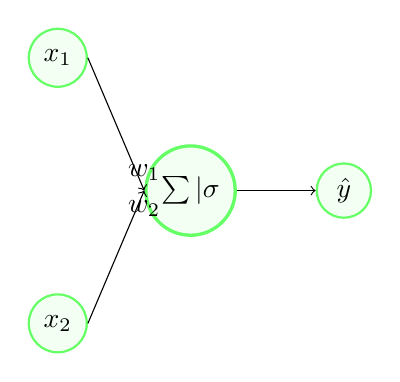
\begin{tikzpicture}[roundnode/.style={circle, draw=green!60, fill=green!5, very thick, minimum size=7mm},
  					 roundnodesmall/.style={circle, draw=green!60, fill=green!5, thick, minimum size=1mm}]
    % Node
    \node[roundnode] (circle) {$\sum | \sigma$};
    \node[roundnodesmall] (x1) [above left=of circle] {$x_1$};
    \node[roundnodesmall] (x2) [below left=of circle] {$x_2$};
    \node[roundnodesmall] (y) [right=of circle] {$\hat{y}$};
    % Lines
    \draw[->] (x1.east) -- (circle.west) node[left,above] {$w_1$};
    \draw[->] (x2.east) -- (circle.west) node[left,below] {$w_2$};
    \draw[->] (circle.east) -- (y);
   \end{tikzpicture}
  \end{center}
  The usage of backpropagation is very straight forward. Neural networks are representation learning algorithms, which means, that they learn the representation of the data over time, without
  having the need of an expert doing pre-processing of anything. It only needs a valid training and testing dataset, where have ground-truth knowledge of the output of the data. One then leverages
  the forward pass of the algorithm to produce our approximated output.
  % todo: fix tikz graph
  \textbf{Forward pass:}
  \begin{equation}
   \hat{y} = \sigma(\sum_{i=1}^{2}x_iw_i)
  \end{equation}
  After computing the regarding output, one will compare the computed output with the ground-truth output with some kind of error-function, e.g. \textbf{MSE}:
  \begin{equation}
   L(y,\hat{y}) = \frac{1}{N}||y-\hat{y}||_2^2 = \frac{1}{N}\sum_{i=1}^{N}(y_i-\hat{y}_i)^2
  \end{equation}    
  This error is then propagated back, using the chain-rule, through the
  graph to update the weights of the network. This is done in the backward pass.\\
  \textbf{Backward pass:}
  \begin{equation}
   \frac{\partial L}{\partial \hat{y}} = \frac{2}{N}\sum_{i=1}^{N}(y_i-\hat{y}_i)
  \end{equation}
  \begin{equation}
   \frac{\partial \sigma(x)}{\partial x} = \sigma(x)(1-\sigma(x))
  \end{equation}
  \begin{equation}
   \frac{\partial L}{\partial \sum_{i=1}^{2}x_iw_i} = \frac{\partial L}{\partial \hat{y}} \cdot \frac{\partial \hat{y}}{\partial \sum_{i=1}^{2}x_iw_i} = \frac{2}{N}\sum_{i=1}^{N}(y_i-\hat{y}_i) \cdot
   \sigma(\sum_{i=1}^{2}x_iw_i)(1-\sigma(\sum_{i=1}^{2}x_iw_i))
  \end{equation}
 
 % subsection
 \subsection{Backpropagation through time (BPTT)} \label{subsection::bptt}
  
 % subsection
 \subsection{PyTorch} \label{subsection::pytorch}
 \newpage

 % related work
 % section
\section{Image Prediction Architectures} 
 % subsection
 \subsection{LSTM Autoencoder}
  % page 1
  \begin{frame}
   \frametitle{LSTM Autoencoder}
   
   \begin{itemize}
    \item<1-> \glqq Unsupervised Learning of Video Representations using LSTMs\grqq by Srivastava et. al. \cite{Srivastava2015}
    \item<2-> Using the standard LSTM from Hochreiter \& Schmidhuber \cite{Hochreiter1997}
    \item<3-> Autoencoder architecture
    \item<4-> Useful for future image prediction \& image reconstruction
    \item<5-> Typical baseline for newer, more advanced algorithms
   \end{itemize}
   
  \end{frame}
  % page 2
  \begin{frame}
   \frametitle{LSTM Autoencoder}
   
   \begin{figure}[H]
    \includegraphics[width=0.7\textwidth]{../Images/srivastava.png}
    \centering
    \caption{Future image prediction model \citep{Srivastava2015}}
    \label{fig:lstm_architecture}
   \end{figure}
  
  \end{frame}
  % page 3
  \begin{frame}
   \frametitle{LSTM Autoencoder}  
  
   \begin{figure}[H]
    \includegraphics[width=0.7\textwidth]{../Images/srivastava_results_mnist.png}
    \centering
    \caption{Results of MovingMNIST experiment \citep{Srivastava2015}}
    \label{fig:lstm_results_mnist}
   \end{figure}
  
  \end{frame}
 
 % subsection
 \subsection{ConvLSTM Autoencoder}
  % page 1
  \begin{frame}
   \frametitle{ConvLSTM Autoencoder}
   
   \begin{itemize}
    \item<1-> \glqq Convolutional LSTM Network: A Machine Learning Approach for Precipitation Nowcasting\grqq by Shi et. al. \citep{Shi2015}
    \item<2-> Similar to LSTM Autoencoder, but uses ConvLSTM instead
    \item<3-> Outperforms the LSTM Autoencoder
   \end{itemize}
   
  \end{frame}
  % page 2
  \begin{frame}
   \frametitle{ConvLSTM Autoencoder}
   
   \begin{figure}[H]
    \includegraphics[width=1.0\textwidth]{../Images/shi.png}
    \centering
    \caption{Future image prediction model \citep{Shi2015}}
    \label{fig:convlstm_architecture}
   \end{figure}
  
  \end{frame}
  % page 3
  \begin{frame}
   \frametitle{ConvLSTM Autoencoder}
   
   \begin{figure}[H]
    \includegraphics[width=0.7\textwidth]{../Images/shi_results_mnist.png}
    \centering
    \caption{Results of MovingMNIST experiment \citep{Srivastava2015}}
    \label{fig:lstm_architecture}
   \end{figure}  
  
  \end{frame}
 
 % subsection
 \subsection{Spatio-temporal Video Autoencoder}
  % page 1
  \begin{frame}
   \frametitle{Spatio-temporal Video Autoencoder}
   
   \begin{itemize}
    \item<1-> \glqq Spatio-Temporal Video Autoencoder With Differentiable Memory \grqq by Patraucean et. al. \cite{Patraucean2015}
    \item<2->
   \end{itemize}
   
  \end{frame}
  % page 2
  \begin{frame}
   \frametitle{Spatio-temporal Video Autoencoder}
   
   \begin{figure}[H]
    \includegraphics[width=1.0\textwidth]{../Images/patraucean.png}
    \centering
    \caption{Spatio-temporal Video Autoencoder Architecture \citep{Patraucean2015}}
    \label{fig:spatiotemp_architecture}
   \end{figure}
  
  \end{frame}
  % page 3
  \begin{frame}
   \frametitle{Spatio-temporal Video Autoencoder}  
  
   \begin{figure}[H]
    \includegraphics[width=0.55\textwidth]{../Images/patraucean_results_mnist.png}
    \centering
    \caption{Results of MovingMNIST experiment \citep{Patraucean2015}}
    \label{fig:lstm_architecture}
   \end{figure}  
  
  \end{frame}
 
 % subsection
 \subsection{PredNet}
  \begin{frame}
   \frametitle{PredNet}
   
  \end{frame}
  
 % subsection
 \subsection{PredRNN}
  \begin{frame}
   \frametitle{PredRNN}  
  
  \end{frame}

 \newpage
 
 % algorithm
 % section
\section{Implementation} \label{section::implementation}
 This section describes the structure and usage of the implemented image-/video-prediction architectures (Shi et al. \cite{Shi2015}, Patraucean et al. 
 \cite{Patraucean2015}, Lotter et al. \cite{Lotter2016}), so that the reader is able to understand the given code and is able to redo the experiments and even 
 extend the code to his own needs.
  
 % subsection
 \subsection{Structure} \label{subsection::structure}
  The code is structured in a way, that everyone without specific knowledge of coding should be able to get the necessary files and results as easy as possible 
  and everyone with more experience in coding should have a nice structure to add or remove certain methods.
  \\\\
  The first important files are the setup.py and requirements.txt. Both of them are useful to install every necessary requirement to run the code on someones 
  local machine or on any machine learning cloud computing platform. This was tested during the experiments on a private computer, on 
  \href{www.floydhub.com} {Floydhub} and \href{colab.research.google.com}{Google Colab}.
  For Google Colab one needs to add a Jupyter notebook file \cite{Kluyver2016}, which is not included in the thesis.
  \\\\
  The part where all comes together is the main file in the PredNet folder, in which the main method is started. This main method controls the whole
  execution, such as initializing the network,
  initializing the optimizer (Adam \cite{Kingma2015} or RMSProp \cite{Ruder2016}) and starting the training or testing. Testing, training and validation 
  are seperated in own files, so the user has more 
  control over the methods itself (For example, the user wants to validate on more then one error, but wants to test on only one, he can simply
  add the change to the validation file, without interchanging with any other method.).
  \\
  Everything related to the actual network models is stored in the model 
  folder, which stores the three baselines and the folder for all submodules of which they consist (For example, PredNet consist of an error module, which is 
  therefore stored in model/modules/error.py.).
  Many useful methods, e.g. the choice of a certain error function can be found in the helper folder. The dataset files are stored in 
  data, as well as some simple scripts to fetch and pre-process the data. Some of this scripts are not written by the thesis author (All files written by the 
  author himself have a tag at the top of the file.). There is also the dataset folder, which holds the \href{https://pytorch.org/docs/stable/
  data.html}{PyTorch dataloader} files.
  \\
  The code is able to save and load model parameters, so one is able to continue training at a certain point, or test the network
  after training. Those network files are stored in the mdl folder.
  \\\\
  To overcome the problem of having the need to change network parameters (Such as depth, kernel sizes, padding sizes, etc.) always inside the
  code files, the implementation offers a solution to the user, where he needs to add \href{https://yaml.org/}{yml}-files which contain every necessary 
  information about the network parameters, where to store the model and the logs, using debug mode and where the dataset files are stored.\\
  The files used for the experiments in section~\ref{section::experiments} are already included, so the user is able to use them as template to create own custom
  designed networks from it. Those files are stored in the yml 
  folder.
  \\\\
  To log the training, validation and test results, the code is using Tensorboard \cite{tensorflow2015}. Those files are stored in the log folder.
  Lastly, the user is able to create the backpropagation graph from the used network. This is outputted into the graph folder. Example backpropagation graphs
  are given in the appendix~\ref{section::appendix}.
  A tree graph of the structure and a simple class and package diagram is also given in the appendix~\ref{section::appendix}.
  
 % subsection
 \subsection{Usage}
  The user starts by fetching the code using git\footnote{Github: \href{https://github.com/dittr/Bachelorthesis}{https://github.com/dittr/Bachelorthesis}}.
  Then it is recommended to use a virtual python environment, that the necessary requirements for running the code doesn't interchange with any python package
  already running on the users environment.
  \\\\
  As described in section~\ref{subsection::structure}, the first important files to look at, are requirements.txt and setup.py. Both of them have the ability to
  install the necessary requirements. For the requirements.txt file, the user simply types:
  \begin{lstlisting}[language=bash]
   python3 -m pip install --user -r requirements.txt
  \end{lstlisting}\noindent
  This simple command inserted into the command line will download all necessary frameworks and libraries for the implementation.
  Another way is to use the setup.py, where the user does:
  \begin{lstlisting}[language=bash]
   python3 setup.py install
  \end{lstlisting}\noindent
  Please note, that the setup.py will install the given code as own package, so if only downloading the requirements is necessary, this solution is preferred.
  After installing all necessary requirements, the user is able to create its own yml-files for the different network parameter.
  As written above, the used yml-files are already included, so if the user only want's to verify the experiments, one doesn't need to change the files.
  \\\\
  Then the user is able to start and run the code.
  This is done using the main.py file, where the first run should look like:
  \begin{lstlisting}[language=bash]
   python3 main.py --help
  \end{lstlisting}\noindent
  This will give the user an overview of all mandatory and optional command line parameters. An example output of this is given in the 
  appendix~\ref{section::appendix}, as well as some example listings of possible training and testing commands.
  \\\\
  The code is using Tensorboard for the error log during training and testing and also the image output during validation and testing, so to be able to use
  this tensorboard, the user should enter:
  \begin{lstlisting}[language=bash]
   tensorboard --logdir=log
  \end{lstlisting}\noindent
  If the user is using e.g. Arch Linux, this could lead to the problem, that tensorboard is not defined. An easy fix for this is:
  \begin{lstlisting}[language=bash]
   alias tensorboard='python3 -m tensorboard.main'
  \end{lstlisting}\noindent
 \newpage
 
 % usage
 % section
\section{Methodology} \label{section::methodology}
 The
 \newpage
 
 % training
 % section
\section{Training} \label{section::training}
The training section will cover the aspects of different training types.
 \newpage
 
 % experiments
 % section
\section{Experiments} \label{section::experiments}
 This section describes the experiments performed on the three implemented networks and the experimental results. The experiments were performed, to see 
 if the implemented networks are able to perform better, when changing the recurrent module with a more advanced recurrent module. The sections starts with 
 the description of the experimental setup, followed by the experimental results.
 
 % subsection
 \subsection{Experimental Setup} \label{subsection::exp_setup}
  The experiments were performed on three different datasets. Initial experiments are performed on a synthetic dataset. This has the advantage of having full 
  knowledge
  about the underlying structure of the data and that one has, in theory, an infinite amount of data for training and testing. This is a very common approach
  and performed in all papers, compared in section~\ref{section::related}.
  \\\\
  MovingMNIST is used as the synthetic dataset, which is a dataset created using handwritten digits from the famous handwritten dataset MNIST
  \cite{LeCun1998}. The idea is to use a pre-defined number of digits, which are spawned at a random position inside a given frame. Those digits are then moved 
  through the frame, given a velocity and momentum. If a digit will touch the boundary of the frame, the digit will bounce back.
  \\\\  
  The other two used datasets are real datasets\footnote{Camera images or videos from the real world.}.
  The first one is KTH \cite{Schuldt2004}, an action recognition dataset, which consists of videos where people
  do different actions, such as hand waving, running and jogging. The second one is Kitti \cite{Geiger2013}, which is an autonomous driving dataset, where
  the authors drove a car through different areas in Karlsruhe, Germany. For example through residential areas and the city.
  \\\\
  MovingMNIST is pre-processed to have a frame size of $(1 \times 64 \times 64)$, two digits per frame and ten frames per sequence.
  The training set consists of $10000$ sequences and the test set of $3000$ sequences.\\
  KTH was pre-processed to gray-scaled images and cropped to the frame size $(1 \times 80 \times 60)$.\\
  Kitti was also cropped to a specific frame size $(3 \times 160 \times 128)$.
  \\\\
  For the first experiments there are several fixed hyperparameters, simply because the network already needs several hours to train, so hyperparameter 
  optimization was not intended, because it would have blown the experiments by a wide margin.
  The amount of epochs and iterations per dataset are fixed as well, as well as using image normalization and having MSE as the
  error function for training and testing.
  \\\\
  For MovingMNIST, it was used one epoch with $5000$ iterations, for KTH $20$ epochs with $500$ iterations per epoch and for Kitti $50$ epochs with $500$ 
  iterations per epoch. The values for MovingMNIST are inspired by Elsayed et al. \cite{Elsayed2018}, where they develop a novel ConvLSTM module for PredNet and 
  train PredNet on the MovingMNIST dataset (Which is not done by the PredNet authors.).
  The values for KTH and Kitti are inspired by Lotter et al. \cite{Lotter2016}.
  In the PredNet paper the authors use $150$ epochs with $500$ iterations per epoch to train PredNet on Kitti dataset, but here the amount of epochs is reduced to
  $50$ because the training would otherwise take more then $20$ hours, which was not applicable for this thesis. Because KTH is a more \glqq simple\grqq dataset 
  (Only 
  objects in the scenery are moving, not the scenery as in Kitti.), the epoch size was artificially chosen to be $20$.
  \\\\
  Adam \cite{Kingma2015} was used as optimizer for all networks, always with the same learning rate of $0.001$, and the same learning rate scheduler (Dividing the 
  learning rate by factor ten after $50$\% of epochs.), even tho 
  Patraucean et al. \cite{Patraucean2015} are using RMSProp \cite{Ruder2016}, in their paper, as optimizer and a different learning rate scheduler.
  The values are used by Lotter et al. \cite{Lotter2016} for PredNet and they were chosen as the hyperparameter for this experiment.
  \\\\
  All other parameters, such as kernel-size, padding-size, channel, depth, etc. can be found in the implementation, in the yml-folder.  
  \\\\
  For the second experiments hyperparameter optimization, early stopping and used \glqq optimal values\grqq given by the authors in the papers was added,
  to show that using those important topics can totally change a decision.
  Due to the complexity and effort of the training of those complex neural network, it was decided to only show one example of the second experiments.
  
 % subsection
 \subsection{Experimental Results (First setup)} \label{subsection::exp_results}
  This section is divided into the three different datasets and all subsections are structured the same way. It starts by comparing the amount of paramters
  for the dataset, because the amount of parameters is directly correlated to the computing time the network needs for training and testing. It then shows
  examples of the testing output and a table of mean MSE error.
  The number of parameters directly correlates to the performance\footnote{In computer science, the performance directly correlates with the computing time.}, 
  therefore is a smaller amount always better, because the network will train faster and is also faster at test time. A tree graph of the performed experiments
  can be found in the appendix~\ref{section::appendix}.
  
  % subsubsection
  \subsubsection{MovingMNIST}
   \begin{table}[H]
    \begin{center}
     \begin{tabular}{| l | l | l |}\hline
      \textbf{Model} & \textbf{ConvLSTM} & \textbf{PredRNN} \\\hline
      Autoencoder (Depth $2$) & $537.411$ & $773.018$ \\\hline
      PredNet & $6.909.818$ & $12.421.090$ \\\hline
      Spatiotemp & $1.001.324$ & $1.415.639$ \\\hline
     \end{tabular}
    \end{center}
    \caption{Number of trainable parameter for MovingMNIST.}
   \end{table}\noindent
   We can clearly see, that the networks using PredRNN, due to it's more complex architecture, has at least $~1.41$ times the amount of parameters. In the worst
   case, here for PredNet (Because PredNet has the PredRNN module in every layer.), the value is $~1.8$. This results show, that the networks using PredRNN
   should perform better in the test to be the superior architecture, because otherwise they don't have any advantage to the architecture using ConvLSTM.
   \begin{figure}[H]
    \includegraphics[width=0.45\textwidth]{../Images/prednet_mnist_training.png}
    \centering
    \caption{Training PredNet with ConvLSTM (blue) and PredRNN (red) on MovingMNIST.}
    \label{fig:prednet_mnist_training}
   \end{figure}\noindent
   \begin{figure}[H]
   \centering
   \subfloat[Ground truth]{{\includegraphics[width=0.6\textwidth]{../Images/prednet_mnist_groundtruth.png} }} 
   \qquad
   \subfloat[ConvLSTM]{{\includegraphics[width=0.6\textwidth]{../Images/prednet_mnist_convlstm_prediction.png} }} 
   \qquad
   \subfloat[PredRNN (vanished)]{{\includegraphics[width=0.6\textwidth]{../Images/prednet_mnist_predrnn_prediction.png} }}
   \caption{Test results for PredNet on MovingMNIST.}
   \label{figure::prednet_mnist_results}
  \end{figure}\noindent
  Here one can see a problem, that was always present during training. The values for MovingMNIST were vanishing very fast, which often resulted in empty images,
  for ConvLSTM and PredRNN. This is due to the fact, that PyTorch is vanishing gradients faster then Keras \cite{chollet2015}, and that Lotter et al. used 
  Matplotlib \cite{Hunter2007}, which is able to catch much smaller values then Tensorboard is (I had to multiply the values with factor ten, to even get some
  output.).
   \begin{table}[H]
    \begin{center}
     \begin{tabular}{| l | l | l |}\hline
      \textbf{Model} & \textbf{ConvLSTM} & \textbf{PredRNN} \\\hline
      Autoencoder (Depth $2$) & $0.027$ & $0.028$ \\\hline
      PredNet & $0.035$ & $0.041$ \\\hline
      Spatiotemp & $0.024$ & $0.022$ \\\hline
     \end{tabular}
    \end{center}
    \caption{Mean MSE for MovingMNIST.}
   \end{table}\noindent
   Those values directly show, that the change from ConvLSTM to PredRNN does not make any positive difference for any network performing the tests on MovingMNIST.
   Therefore, as written above, the network using PredRNN only consist of more parameter, so the choice should therefore tend to ConvLSTM, because it has less
   computing time and similar results.
   
  % subsubsection
  \subsubsection{KTH}
   \begin{table}[H]
    \begin{center}
     \begin{tabular}{| l | l | l |}\hline
      \textbf{Model} & \textbf{ConvLSTM} & \textbf{PredRNN} \\\hline
      Autoencoder (Depth $2$) & $542.531$ & $781.760$ \\\hline
      PredNet & $850.325$ & $1.285.730$ \\\hline
      Spatiotemp & $1.007.598$ & $1.421.913$ \\\hline
     \end{tabular}
    \end{center}
    \caption{Number of trainable parameter for KTH.}
   \end{table}\noindent
   \begin{figure}[H]
   \centering
   \subfloat[Ground truth]{{\includegraphics[width=0.6\textwidth]{../Images/prednet_kth_groundtruth.png} }} 
   \qquad
   \subfloat[ConvLSTM]{{\includegraphics[width=0.6\textwidth]{../Images/prednet_kth_convlstm.png} }} 
   \qquad
   \subfloat[PredRNN]{{\includegraphics[width=0.6\textwidth]{../Images/prednet_kth_predrnn.png} }}
   \caption{Test results for PredNet on KTH.}
   \label{figure::prednet_kth_results}
  \end{figure}\noindent
   \begin{table}[H]
    \begin{center}
     \begin{tabular}{| l | l | l |}\hline
      \textbf{Model} & \textbf{ConvLSTM} & \textbf{PredRNN} \\\hline
      Autoencoder (Depth $2$) & $1.55e-3$ & $0.05$ (didn't converged) \\\hline
      PredNet & $1.95e-3$ & $1.93e-3$ \\\hline
      Spatiotemp & $3.1e-3$ & $0.025$ (didn't converged) \\\hline
     \end{tabular}
    \end{center}
    \caption{Mean MSE for KTH.}
   \end{table}
  
  % subsubsection
  \subsubsection{Kitti}
   \begin{table}[H]
    \begin{center}
     \begin{tabular}{| l | l | l |}\hline
      \textbf{Model} & \textbf{ConvLSTM} & \textbf{PredRNN} \\\hline
      Autoencoder (Depth $2$) & $542.531$ & $781.760$ \\\hline
      PredNet & $8.222.559$ & $12.430.626$ \\\hline
      Spatiotemp & $1.640.321$ & $2.200.641$ \\\hline
     \end{tabular}
    \end{center}
    \caption{Number of trainable parameter for Kitti.}
   \end{table}\noindent
   \begin{figure}[H]
   \centering
   \subfloat[Ground truth]{{\includegraphics[width=0.7\textwidth]{../Images/prednet_kitti_groundtruth.png} }} 
   \qquad
   \subfloat[ConvLSTM]{{\includegraphics[width=0.7\textwidth]{../Images/prednet_kitti_convlstm.png} }} 
   \qquad
   \subfloat[PredRNN]{{\includegraphics[width=0.7\textwidth]{../Images/prednet_kitti_predrnn.png} }}
   \caption{Test results for PredNet on Kitti.}
   \label{figure::prednet_kth_results}
  \end{figure}\noindent
   \begin{table}[H]
    \begin{center}
     \begin{tabular}{| l | l | l |}\hline
      \textbf{Model} & \textbf{ConvLSTM} & \textbf{PredRNN} \\\hline
      Autoencoder (Depth $2$) & $0.02$ & $0.013$ \\\hline
      PredNet & $0.019$ & $0.02$ \\\hline
      Spatiotemp & $0.018$ & $0.017$ \\\hline
     \end{tabular}
    \end{center}
    \caption{Mean MSE for Kitti.}
   \end{table}\noindent
 \\\\
 The experiments showed, that using this kind of setup, the PredRNN as recurrent module does not lead to a significant performance boost, but instead only
 increases the number of trainable parameter. Therefore, using this setup, PredRNN is not the superior sub-module and should not be used. But, as this experiments
 are performed with any kind of hyperparameter optimization, this results are not valid to make a real decision if PredRNN is really not superior to the standard
 ConvLSTM module.

 % subsection
 \subsection{Experimental Results (Second setup)} \label{subsection::second_exp}
  This test was only performed on the KTH dataset, with an optimal learning rate of $0.0001$ for the Autoencoder.
  \begin{figure}[H]
   \includegraphics[width=0.6\textwidth]{../Images/exp2_training_error.png}
   \centering
   \caption{Training Autoencoder with ConvLSTM (red) and PredRNN (gray) on KTH using hyperparameter optimization and early stopping.}
   \label{fig:autoenc_exp2_training}
  \end{figure}\noindent
  The mean test mse error for the Autoencoder using the standard ConvLSTM module is: $0.0013$ and for the Autoencoder using the PredRNN module: $0.00072$.
  This means, that PredRNN was able to boost the performance of the Autoencoder by more then $80$ percent.
  \begin{figure}[H]
   \centering
   \subfloat[Ground truth]{{\includegraphics[width=0.65\textwidth]{../Images/exp2_test_ground.png} }} 
   \qquad
   \subfloat[ConvLSTM]{{\includegraphics[width=0.1\textwidth]{../Images/exp2_test_convlstm.png} }} 
   \qquad
   \subfloat[PredRNN]{{\includegraphics[width=0.1\textwidth]{../Images/exp2_test_predrnn.png} }}
   \caption{Test results for Autoencoder on KTH using hyperparameter optimization and early stopping.}
   \label{figure::prednet_mnist_results}
  \end{figure}\noindent
  This experiment showed the importance of hyperparameter optimization and early stopping and why it should be used always in terms of learning neural networks.
  A more explicit analysis of this result is given in the discussion~\ref{section::discussion}.
 \newpage
 
 % discussion
 % section
\section{Discussion} \label{section::discussion}

 \newpage
 
 % conclusion
 % section
\section{Conclusion} \label{section::conclusion}
 The thesis showed different approaches for image-/video-prediction and how important the choice of the recurrent sub-module is.
 First the reader got an extensive introduction
 about all necessary topics, which were necessary to fully understand the following chapters. Then the thesis gave a comprehensive related work part, in which
 five state-of-the-art image-/video-prediction algorithms are described, by showing the architecture and the results of the experiments of the synthetic dataset.
 This five architectures showed, how different the approaches for image-/video-prediction are, but also how similar in form of
 having a similar recurrent module and some using a type of autoencoder architecture.
 \\\\
 Because the re-implementation
 of the three baselines is a big part of this bachelor thesis, the implementation chapter described how the code is structured and how to use the code, so any
 user (with minimal knowledge of PyTorch / neural networks) is able to use and possibly adapt the code for validating the performed experiments or even perform
 own further experiments. Then the reader got the methodology, in which the way how the experiments are performed is described in-depth, so the reader will 
 understand the key-aspects of the experiments.
 \\\\
 The experimental results were given in the experiments section.
 The experiments showed, how important the right choice of a recurrent module is and also how important hyperparameter optimization is in training neural networks.
 The first experiments were performed using static settings for all network implementations. Those experiments showed, that without using the \glqq best\grqq 
 hyperparameters for each network, the choice of a more advanced recurrent module is not necessary.
 \\\\ 
 After performing hyperparameter optimization and using given \glqq optimal\grqq values 
 from the implemented papers, even one example already showed that
 PredRNN should be the superior module and should be tested again in all implemented architectures. 
 Lastly, there is the discussion in which
 the reader gets an interpretation of the experimental results and how they affect image-/video-prediction neural networks.
 \\\\
 For future experiments, it would be awesome to see the hyperparameter optimization performed for all $18$ test cases and if PredRNN is able to outperform
 the standard ConvLSTM module in all of the tests.
 
 % Explanation of self written thesis
 Erklärung über das selbstständige Verfassen von \glqq Comparing different state-of-the-art solutions for image prediction using time-series analysis\grqq\\
Ich versichere hiermit, dass ich die vorstehende Bachelorarbeit selbständig verfasst und keine anderen als die angegebenen Hilfsmittel benutzt habe. Die Stellen der obigen Arbeit, die anderen Werken dem Wortlaut oder dem Sinn nach entnommen wurden, habe ich in jedem einzelnen Fall durch die Angabe der Quelle bzw. der Herkunft, auch der benutzten Sekundärliteratur, als Entlehnung kenntlich gemacht. Dies gilt auch für Zeichnungen, Skizzen, bildliche Darstellungen sowie für Quellen aus dem Internet und anderen elektronischen Text-und Datensammlungen und dergleichen. Die eingereichte Arbeit ist nicht anderweitig als Prüfungsleistung verwendet worden oder in deutscher oder in einer anderen Sprache als Veröffentlichung erschienen. Mir ist bewusst, dass wahrheitswidrige Angaben als Täuschung behandelt werden.\\\\
Datum, Ort Unterschrift\\ 
 
 % literature
% \newpage
% \pagestyle{empty}
 \pdfbookmark[section]{Bibliography}{Bibliography}
 \bibliography{../Bibliography/bibliography.bib} \label{section::literature}

\end{document} 
 
